\documentclass[xcolor=dvipsnames]{beamer} 
%\usecolortheme[named=Plum]{structure}
\usecolortheme[named=OliveGreen]{structure} 
%\usecolortheme[named=Green]{structure} 
%\usecolortheme[named=Apricot]{structure}
%\usecolortheme[named=Red]{structure}
%\usecolortheme[named=Blue]{structure}
%\usecolortheme[named=Lily]{structure}
\useoutertheme{infolines} 
\usetheme[height=7mm]{Rochester} 
\setbeamertemplate{items}[ball] 
\setbeamertemplate{blocks}[rounded][shadow=true] 
\setbeamertemplate{navigation symbols}{} 

\mode<presentation>
{
%\usetheme{default}
%\usetheme{Berkeley}
\usetheme{Warsaw}
%\setbeamercovered{transparent}
%\usetheme{AnnArbor}
%\usetheme{Antibes}
%\usetheme{Bergen}
%\usetheme{Hannover}
%\usetheme{Marburg}
%\usetheme{Montpellier}
%\usetheme{PaloAlto}
}

%%
\usepackage[english]{babel}
\usepackage[utf8]{inputenc}
\usepackage{times}
\usepackage[T1]{fontenc}
\usepackage{colortbl} 
\usepackage{algorithm}
%\usepackage{algpseudocode}
%\usepackage{algorithmic}
%\usepackage[ruled,lined,boxed,commentsnumbered]{algorithm2e}
\usepackage{subfigure}
\title[Slide Number\hspace{2em}\insertframenumber]
%/\inserttotalframenumber]
{SAT-attack Resilient Sequential Locking}
\subtitle
{}
\author[]
{Seetal Potluri}
\institute[Universities]
{
    Chair for Processor Design, Technical University of Dresden
}


\subject{Deep Submicron Digital VLSI Design}
 
 
%\pgfdeclareimage[height=1.25cm]{iitmlogo}{iitmlogo}
%\logo{\pgfuseimage{iitmlogo}}


\AtBeginSubsection[]
{
\begin{frame}<beamer>{Outline}
\tableofcontents[currentsection,currentsubsection]
\end{frame}
}


\begin{document}


\begin{frame}
\titlepage
\end{frame}


\begin{frame}{Outline}
\tableofcontents
% You might wish to add the option [pausesections]
\end{frame}

\section{Motivation}
\section{Motivation}

Figure~\ref{fig:c432-logic-encrypted-observe-flops} shows the implementation of a logic-encrypted version of \texttt{c432} circuit, with observe flip-flops at the primary outputs.  
\begin{figure}[!htbp]
	\centering
	\includegraphics[scale=0.3]{fig/c432-sequential}
	\caption{Logic encrypted \texttt{c432} circuit, with observe flip-flops}
	\label{fig:c432-logic-encrypted-observe-flops}
\end{figure}


\section{Attack and Access models}
\begin{frame}{Attack model}
\begin{itemize}
\item The encryption key is stored in tamper-proof memory, so not available; 
\item The attacker has access to layout and mask information from a malicious foundry. The gate-level netlist can be reverse engineered from this;  and 
\item The attacker has access to an activated IC on which to apply input patterns and observe outputs. This could be obtained by purchasing an activated IC from the open market\footnote{P. Subramanyan et al, "Evaluating the Security of Logic Encryption Algorithms", HOST 2015}. 
\end{itemize}
\end{frame}

\begin{frame}{Access model}
\begin{itemize}
\item The attacker applies inputs to the circuit through the DFT architecture; 
\item In general, the IC vendor keeps test (scan) mode alive even after testing, for the purpose of debugging customer returns \footnote{S. Mitra et al, "Robust system design with built-in soft-error resilience", IEEE Computer, 2005.} \footnote{A. Carbine et al, "Pentium Pro Processor Design for Test and Debug", ITC 1997} (customer returned chips, are debugged for yield learning); 
\item Another reason why scan is not deactivated, so that customer can apply his test patterns and test for quality themselves. 
\item Mode of DFT operation for launching SAT-attack: EDT-BYPASS.
\end{itemize}
\end{frame}

%\section{Design for Testability (DFT)}
\begin{frame}{Design for Testability (DFT)}
\begin{itemize}
\item Prevalently used to improve controllability/observability 
\item Industry DFT standard: Scan
\item Industry DFT Compression standard: Embedded Deterministic Test (EDT)
\end{itemize}
\end{frame}

\begin{frame}{Normal Circuit}
\begin{figure}
\begin{center}
\label{fig:scan-insertion}
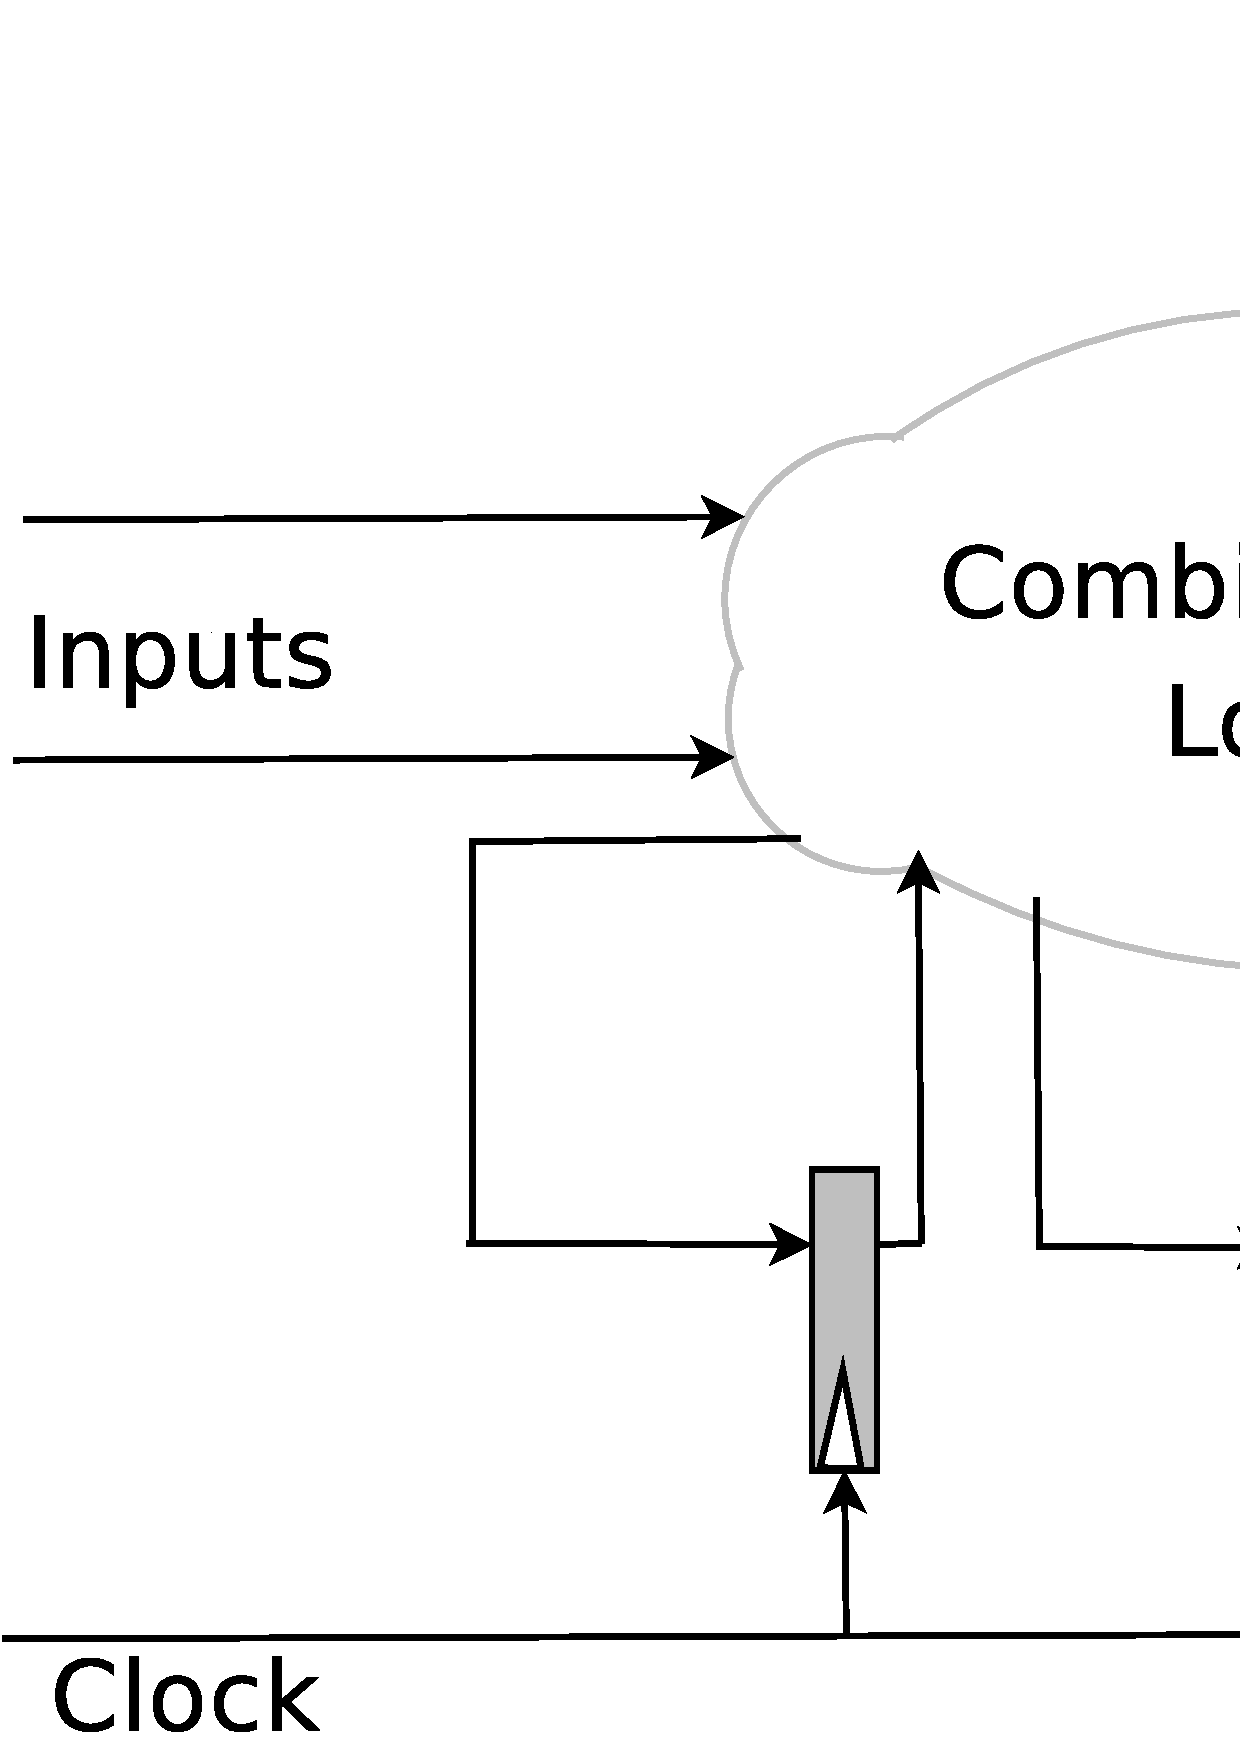
\includegraphics[scale=0.2]{fig/normal_circuit.pdf}
\end{center}
\end{figure}
\end{frame}

\begin{frame}{Circuit with Scan Insertion}

	\only<+>{
		\begin{figure}
		\begin{center}
		\label{fig:scan-insertion}
		\includegraphics[scale=0.2]{fig/scan_inserted_circuit.pdf}
		\end{center}
		\end{figure}
	}
	\only<+>{
		\begin{figure}		
		\begin{center}
		\caption{Shift mode}
		\label{fig:shift-mode}
		\includegraphics[scale=0.2]{fig/scan_inserted_circuit_shift_mode.pdf}
		\end{center}
		\end{figure}
	}
	\only<+>{
		\begin{figure}
		\begin{center}
		\caption{Capture mode}
		\label{fig:capture-mode}
		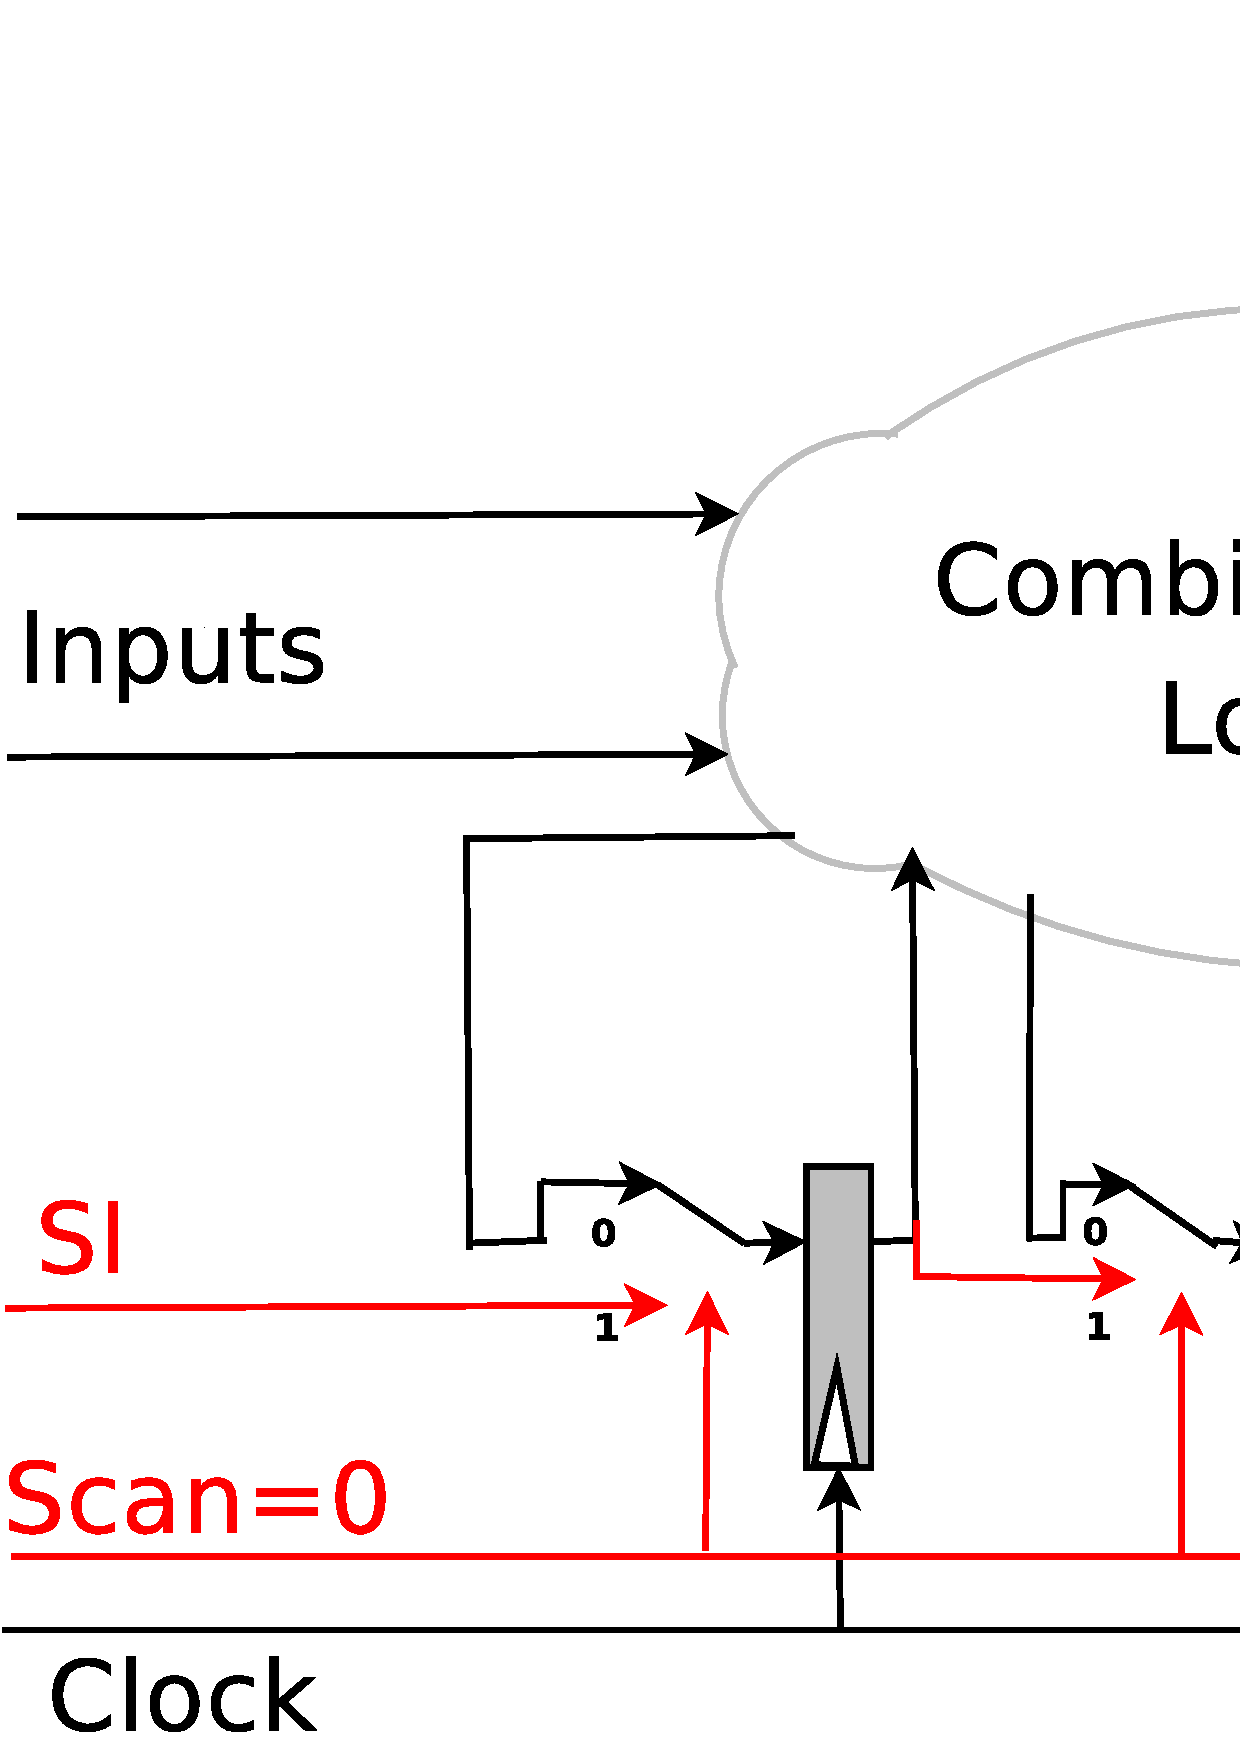
\includegraphics[scale=0.2]{fig/scan_inserted_circuit_capture_mode.pdf}
		\end{center}
		\end{figure}
	}
\end{frame}


\begin{frame}{Circuit with EDT Insertion}
\begin{figure}
\begin{center}
\label{fig:scan-mode}
\includegraphics[scale=0.2]{fig/EDT.pdf}
\end{center}
\end{figure}
\end{frame}



\section{Sequential Locking}
%\section{DFT Encryption}
\begin{frame}{Modes of EDT Operation, SAT-attack}
\begin{itemize}
	\item EDT-mode : Not possible to launch the SAT-attack in this mode, since not possible to assign every scan cell to desired value 
	\item EDT-BYPASS-mode : Possible to launch the SAT-attack in this mode, since all scan cells are daisy-chained and directly accessible
\end{itemize}
\end{frame}

\begin{frame}{DFT Encryption}
\alert{Idea:} Encrypt DFT path corresponding to the EDT-BYPASS mode, to make sequential circuit resilient to SAT-attack
\end{frame}

\begin{frame}{DFT Encryption}
\begin{figure}
\begin{center}
\label{fig:encrypted-dft}
\includegraphics[scale=0.2]{fig/encrypted-DFT.pdf}
\end{center}
\end{figure}
\end{frame}

\begin{frame}{Libary Scan Cell}
\begin{figure}
\begin{center}
\label{fig:sc}
\includegraphics[scale=0.2]{fig/traditional-scanflop.pdf}
\end{center}
\end{figure}
\end{frame}

\begin{frame}{Existing Encrypted Scan Cell}
\begin{figure}
\begin{center}
\label{fig:encrypted-sc}
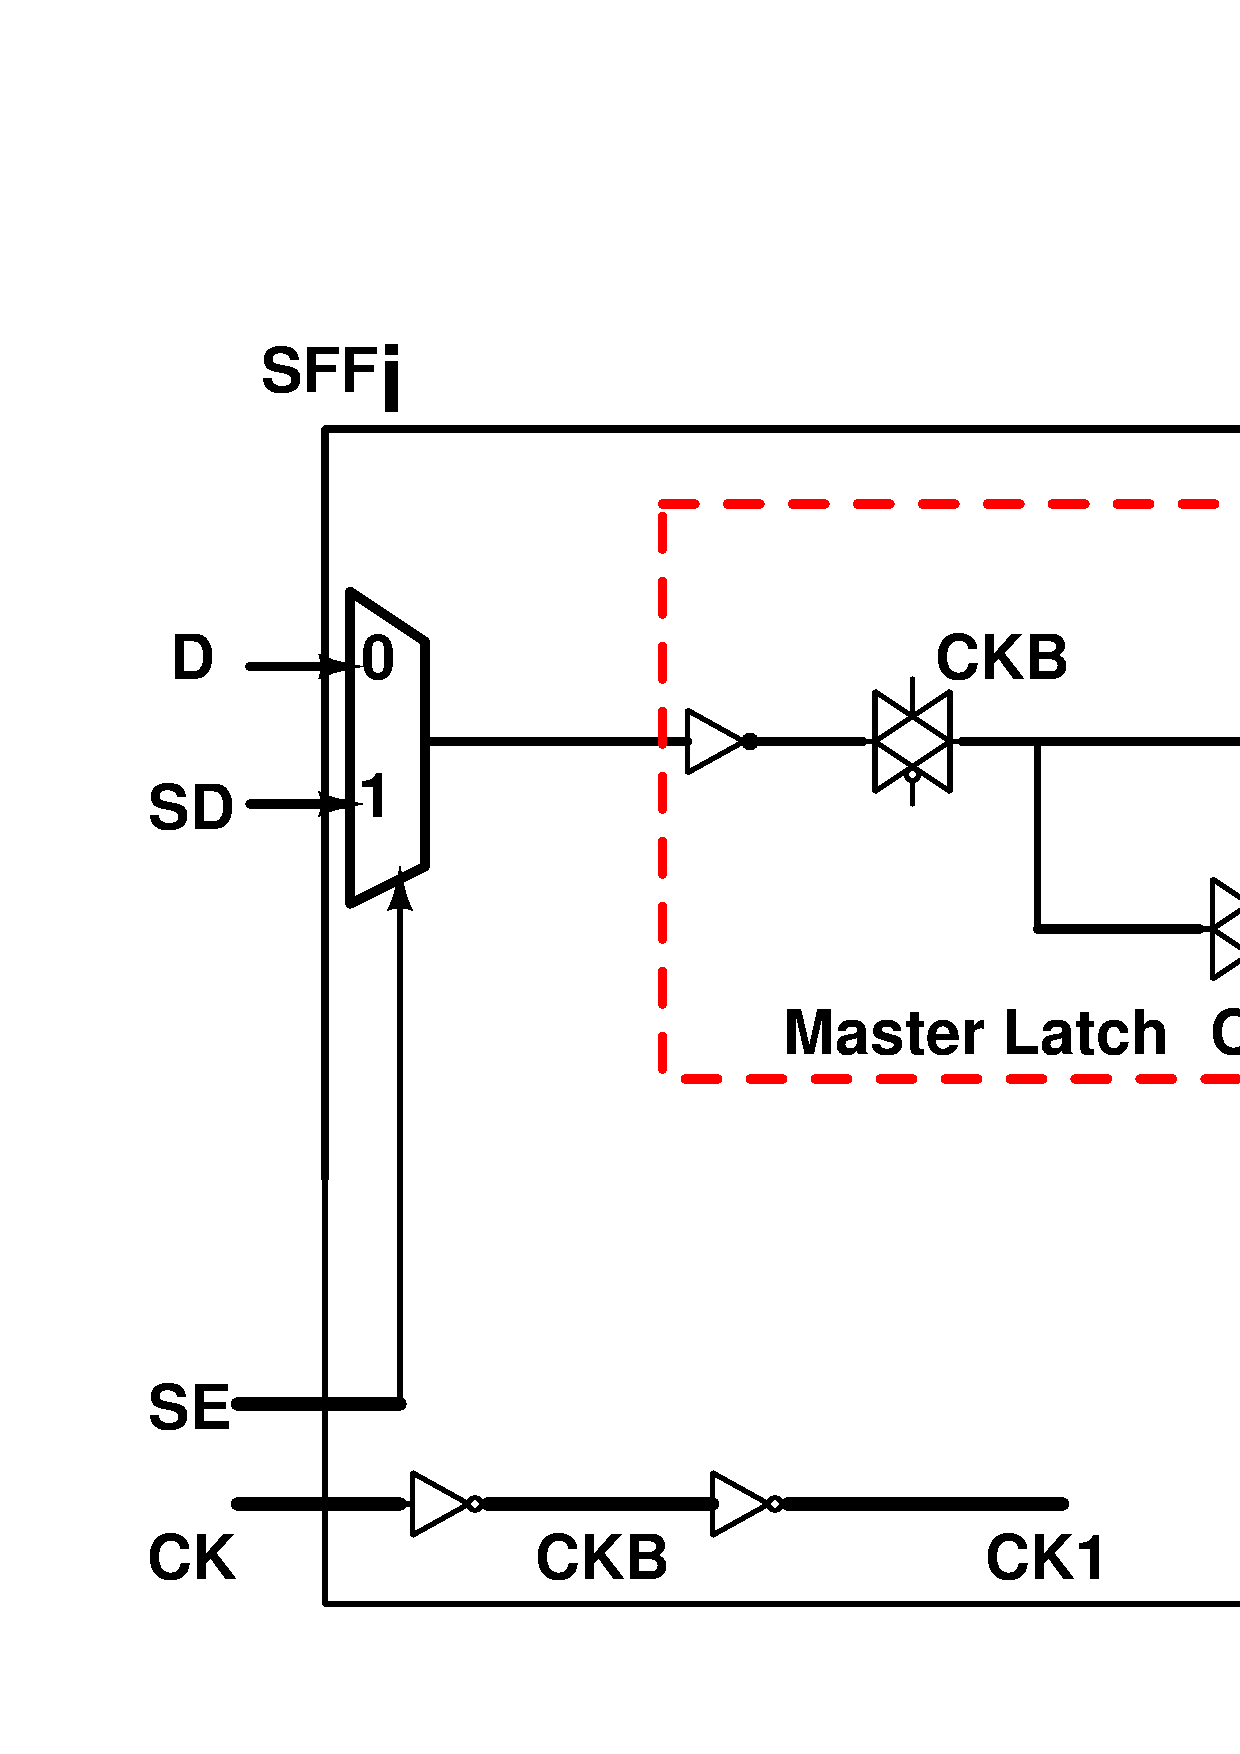
\includegraphics[scale=0.2]{fig/encrypted-scanflop.pdf}
\caption{It is possible to decrypt the correct key\footnote{L. Alrahis, "ScanSAT: Unlocking Obfuscated Scan Chains", ASP-DAC 2019}}
\end{center}
\end{figure}
\end{frame}

\begin{frame}{Proposed Encrypted Scan Cell}
\begin{figure}
\begin{center}
\label{fig:encrypted-sc}
\includegraphics[scale=0.2]{fig/encrypted-scanflop-2.pdf}
\caption{Only combinational portion of the sequential key locks the functional mode of operation}
\end{center}
\end{figure}
\end{frame}


\begin{frame}{SAT attack on Encrypted DFT (BYPASS mode)}
\begin{itemize}
	\item All the scan chains connect together to form 1 single chain
	\item The scan cells can be removed and their inputs/outputs can be unrolled as a function of the XOR gates along the scan-shift path
\end{itemize}
\end{frame}

%\begin{frame}{SAT attack on Encrypted DFT (BYPASS mode)}
%\begin{figure}
%\begin{center}
%\caption{Scan-unrolled circuit }
%\label{fig:encrypted-sc}
%\includegraphics[scale=0.2]{fig/SATattack-on-encrypted-DFT.pdf}
%\end{center}
%\end{figure}
%\end{frame}

\begin{frame}{Example}
\begin{figure}
\begin{center}
\caption{s27 circuit with all scan cells encrypted}
\label{fig:s27}
\includegraphics[scale=0.15]{fig/s27.pdf}
\end{center}
\end{figure}
\end{frame}

\begin{frame}{Example}
\begin{figure}
\begin{center}
\caption{s27 circuit after scan unroll}
\label{fig:s27-after-scan-unroll}
\includegraphics[scale=0.12]{fig/s27_after_scanunroll.pdf}
\end{center}
\end{figure}
\end{frame}

\begin{frame}{Example}
\begin{figure}
\begin{center}
\caption{s27 circuit after scan unroll - SAT overhead}
\label{fig:s27-after-scan-unroll-SAT-overhead}
\includegraphics[scale=0.12]{fig/s27_after_scanunroll_SAToverhead.pdf}
\end{center}
\end{figure}
\end{frame}


\section{Problem Formulation}
\begin{frame}{Tradeoff}
\begin{itemize}
\item The higher the number of scan-cells that are encrypted, the better
%\item Replacing the NOT gate with XOR gate inside the scan-cell incurs area, timing and power overhead
\item The larger the size of the SAT instance, \alert{the harder to decrypt}
\item Encrypting the scan cell incurs \alert{slight area, timing and power overheads}
\item Routing scan-encryption-key bits incur \alert{slight area overhead}
\end{itemize}
\end{frame}


\begin{frame}{Notation}
\begin{block}{Notation}
Define scan-unencrypted circuit $C(G,SC,CK)$ and scan-encrypted circuit $C^{'}(G,SC,CK,SK)$, where \\
$G = \{g_0, g_1, \ldots g_N\}$ is set of gates \\
$SC = \{sc_0, sc_1, \ldots sc_N\}$ is set of scan cells \\
$CK = \{ck_0, ck_1, \ldots ck_X\}$ is the combinational-logic-encryption key and \\
$SK = \{sk_0, sk_1, \ldots sk_Y\}$ is the scan-encryption key \\
\end{block}

\begin{block}{Notation}
	Define $C^{'}_U(G,CK,G_U)$ be the scan-unrolled circuit, where $G_U$ is the list of gates added to $C$ during unroll.
\end{block}

\end{frame}



\begin{frame}{SAT attack on Encrypted DFT (BYPASS mode)}
\begin{table}[!htbp]
\begin{center}
\caption{SAT instance complexity if all SCs encrypted}
\label{tab:allSCs-encrypted}
\begin{tabular}{|c|c|c|c|c|}
\hline
	Benchmark & $|G|$ & $|SC|$ & $|G_U|$ & Increase in SAT \\
		  &          &     &         & instance complexity \\
	\hline
	b17 & 27.99K & 1407 & 2033K & $\approx$ \texttt{72x}\\
	\hline
	b18 & 75.8K  & 3308 & 11451K & $\approx$ \texttt{152x}\\
	\hline 
	b19 & 146.5K & 6618 & 44084K & $\approx$ \texttt{300x}\\
\hline
\end{tabular}
\end{center}
\end{table}
\end{frame}

%\begin{frame}{SAT attack on Encrypted DFT (BYPASS mode)}
%\begin{table}[!htbp]
%\begin{center}
%\caption{SAT instance complexity if first half of SCs encrypted}
%\label{tab:firsthalfSCs-encrypted}
%\begin{tabular}{|c|c|c|c|c|}
%\hline
%	Benchmark & \# $|G|$ & $|SC|$ & $|G_U|$ & Increase in SAT \\
%		  &          &        &         & instance complexity \\
%	\hline
%	b17 & 27.99K & 1407 & 274.74K & $\approx$ \texttt{10x}\\\hline
%	b18 & 75.8K  & 3308 & 1442.83K & $\approx$ \texttt{19x}\\\hline 
%	b19 & 146.5K & 6618 & 5619.59K& $\approx$ \texttt{38x}\\\hline
%\hline
%\end{tabular}
%\end{center}
%\end{table}
%\end{frame}
%
%\begin{frame}{SAT attack on Encrypted DFT (BYPASS mode)}
%\begin{table}[!htbp]
%\begin{center}
%\caption{SAT instance complexity if second half of SCs encrypted}
%\label{tab:secondhalfSCs-encrypted}
%\begin{tabular}{|c|c|c|c|c|}
%\hline
%	Benchmark & $|G|$ & $|SC|$ & $|G_U|$ & Increase in SAT \\
%		  &          &     &         & instance complexity \\
%	\hline
%	b17 & 27.99K & 1407 & 742.25K & $\approx$ \texttt{27x}\\\hline
%	b18 & 75.8K  & 3308 & 4282.75K & $\approx$ \texttt{57x}\\\hline 
%	b19 & 146.5K & 6618 & 16422.56K & $\approx$ \texttt{112x}\\\hline
%\hline
%\end{tabular}
%\end{center}
%\end{table}
%\end{frame}

\begin{frame}{Observations}
\begin{itemize}
%\item Scan-cell encryption resilience depends on the position of the encrypted scan-cell in the scan-chain
\item Let $n=|SC|$
\item Encrypting $i^{th}$ scan-cell in the scan-chain, contributes $i$ XOR gates along scan-out path and $n-i+1$ XOR gates along scan-in path, to $G_U$
\item $(i) + (n-i+1) = n + 1$. So, encrypting any scan-cell in the scan-chain (independent of the position), contributes $n+1$ XOR gates to $G_U$. 
\item Encrypting all scan-cells contributes to $n(n+1)$ XOR gates to $G_U$. 
%\item This is the reason encrypting second half of scan-chain is more effective than encrypting first half of scan-chain
%\item Encrypting scan cells towards end of the chain has multiple benefits
%	\begin{enumerate}
%		\item Since these scan cells are towards the end, they add maximum number of XOR gates to $G_U$, hence adds maximum resilience
%		\item Since these scan cells are towards the end, routing the encryption key bits to them incurs less ovehead
%	\end{enumerate}
\end{itemize}
\end{frame}

\begin{frame}{Observations}
\begin{itemize}
\item Resilience against SAT-attack improves with size of scan-chain
\item For e.g:. if an SoC has {\em 1 million} scan-cells, in EDT-BYPASS mode, all of them form a single-chain. So, just encrypting any one scan cell in the chain will add $\approx ${\em 1 million} XOR gates to the SAT instance, which 
	makes the proposed technique very effective, with minimum overhead. 
\end{itemize}
\end{frame}

\begin{frame}{Problem Formulation}
\begin{block}{Objective}
	Encrypt a subset of scan-cells( in $C$), $SC_E \subset SC \ni$  $\frac{|G + G_U|}{|G|}$ is maximized, while encryption overhead is minimized. 
\end{block}

\end{frame}

%\section{Overhead Evaluation (Proposed Experiments)}
\begin{frame}{Scan cell encryption overhead (proposed experiments) }
\begin{itemize}
\item Replacing NOT gate with XOR gate
\item Incurs slight area, timing and power overheads
\item Can be minimized by transistor sizing
\item \alert{Plan}:
\begin{enumerate}
	\item SPICE simulation to quantify overheads
	\item Use NG-SPICE, FreePDK 45nm Standard library Scan cell and Berkeley 45nm Predictive Technology Model
\end{enumerate}
\end{itemize}
\end{frame}

%\begin{frame}{Scan-encryption Key routing overhead (proposed experiments)}
\begin{itemize}
\item mPL placer \footnote{mPL - A Multilevel Global Placement Tool, URL: http://cadlab.cs.ucla.edu/cpmo/}, takes an initial placement as input and produces a legalized placement as output
\item \alert{Plan}: As already defined, $C$ and $C^{'}$ denote the scan-unencrypted and scan-encrypted netlists respectively, and $SK$ is the scan-encryption key 
\begin{enumerate}
\item run mPL and find placement $P(C)$
\item run mPL and find placement $P(C^{'})$, using $P(C)$ as initial solution
\item Quantify area overhead based on the difference in total area (bounding box) occupied by $P(C^{'})$ and $P(C)$
\end{enumerate}
\end{itemize}
\end{frame}

%%\section{Akash feedback}
\begin{frame}{Akash feedback}
\begin{itemize}
\item Is it necessary for a new work (DFT encryption etc.) in this direction, or is it possible to easily extend Prof. Mallik's work to sequential circuits ?
\item Is it possible to remove combinational logic-locking completely, and do only scan-locking ?
\item Is it possible to remove some key gates in combinational logic, and thereby add keys in scan, so that we can get away without any overhead ?
\item Will the encrypted-scan-cell, in spite of change in cell layout, fit within the standard cell row ?
\item Ensure work-related data is backed-up!
\end{itemize}
\end{frame}

%\begin{frame}{Lockup Latch Encryption}
\begin{itemize}
\item During physical synthesis, negative-level-sensitive lock-up latches are inserted at points in the positive-edge-triggered scan chain, where there are hold-timing-violations; 
\item It is possible to design an encrypted lock-up latch, that functions as positive- or negative-level sensitive, depending on the encryption key bit controlling it; 
\item Insert dummy lock-up latches along with the existing lock-up latches in the scan chain; and 
\item Encrypt all of them and encryption key comes from tamper-proof memory, and the attacker will not know which of them are original and which are dummy, since he cannot perform post-physical-synthesis STA, which is expensive. 
\end{itemize}
\end{frame}

%\begin{frame}{Motivational example on SK routing}
\begin{itemize}
\item \texttt{ibm04} benchmark, die size including pins is 2612x2340; excluding pins is 2602x2321
\item a27189 cell is located at (1810,1121) after detailed placement of ibm04
\item \texttt{ibm04-encrypt} : a27189 cell encrypted using p288 terminal
\item After detailed placement of this encrypted circuit - die size including pins is 2612x2340 (same); excluding pins is 2603x2321
\item So, there is little/no impact for encrypting just one cell. Reason: there is already some spare routing space available
\end{itemize}
\end{frame}

\begin{frame}{Brainstorming}
\begin{itemize}
	\item \alert{Combinational logic encryption - check if somebody has done analysis on routing overhead}
	\begin{enumerate}
		\item How does routing overhead increase with increase in key length ?
		\item Tradeoff between security and routing overhead ?
		\item \texttt{IBM} benchmarks and {\em mPL} can be used for evaluation, setup is ready 
	\end{enumerate}
\item DFT encryption 
	\begin{enumerate}
		\item How does routing overhead increase with increase in key length ?
		\item Tradeoff between security and routing overhead ?
	\end{enumerate}
\end{itemize}
\end{frame}


%\begin{frame}{Devendra's feedback}
\begin{itemize}
\item Scan not deactivated, when giving to customer, so that customer can test for quality. There are different agreements; 
%\item Very difficult to identify positive-edge-triggered flipi-flops from negative-edge-triggered flip-flops unless you know the waveforms; 
\item Design aspect wise, if you mess up with the design by mixing positive-edge-triggered flip-flops with negative-edge-triggered flip-flops or vice-versa, timing will fail and the design will not work; 
\item Why people use both types of flip-flops in same design ? for half-cycle time-borrowing
	\begin{enumerate}
	\item Memory controllers, when memory need to be sampled at both the edges. E.g., DDR
	\item TDO in TDR (TAP controller), where the flip-flops are pulsed at negative-edge; and 
	\item Lock-up latches - negative-level-sensitive ones are used in positive-edge-triggered design.
	\end{enumerate}
\end{itemize}
\end{frame}

%\begin{frame}{Akash feedback on 17.08.2018}
\begin{itemize}
\item Since \alert{Encrypt Flip-Flop} paper already exists, just pushing the XOR gate inside the flip-flop will be very weak contribution, \alert{still we can include because it is novel}
\item Focus on Dummy Lock-up Latch Insertion and encryption of all lock-up latches (both original and dummy)
\item Design an encrypted lock-up latch, which is negative-level-sensitive when control is \alert{0}, and positive-level-sensitive when control is \alert{1}
\item Lock-up latches across (clock) domains are easily understood, so not easy to encrypt. However, lock-up latches within a (clock) domain are not easily understood without detailed clock simulation, hence possible to introduce dummy ones and encrypt to fool the attacker. So, we focus on encryption of lock-up latches within a (clock) domain. 
\end{itemize}
\end{frame}

\begin{frame}{Proposed Experiments (Positive-Edge-Triggered Design)}
	\begin{itemize}
		\item SAT attack has to be launched through EDT BYPASS mode
%		\item Assume Positive-Edge-Triggered design
		\item Since all scan-chains are daisy-chained, surely there will be lot of lock-up latches (because scan chains that are widely spread across SoC are connected, so heavy skew). For these cases, use encrypted lock-up latchwith control=0
		\item Add extra dummy lock-up latches at places where they are not required, however for these cases, use encrypted lock-up latch with control=1
		\item The attacker will not know which are real and which are dummy. 
			\begin{itemize}
				\item \alert{Reason}: Not all far-apart scan-cell-pairs need a lockup latch. So, not easy for attacker to figure out which are real and which are dummy, and hence the correct key. 
			\end{itemize}
	\end{itemize}
\end{frame}

\begin{frame}{Proposed Experiments}
\begin{itemize}
	\item Need placement information of all scan-cells
	\item Currently, have access def files of all ITC benchmarks (without scan cells)
	\item \alert{Assumption}: Consider coordinates of the gate driven by the scan cell, as the coordinate of the scan cell
	\item \texttt{b19} has 6.6K scan cells, so 
	\begin{itemize}
		\item if taking maximum 500 scan cells in one-chain (industry practice), there will be 13 scan-chains
		\item if taking maximum 300 scan cells in one-chain, there will be 22 scan-chains
		\item if taking maximum 100 scan cells in one-chain, there will be 66 scan-chains

	\end{itemize}
\end{itemize}
\end{frame}

\begin{frame}{Proposed Experiments}
\begin{itemize}
	\item Fix maximum chain length to desired value, and use coordinates to cluster them into multiple chains using machine learning. 
	\item Connect the chains successively, through end scan cells. 
	\item Do clock tree simulation (Use Timing book)
	\begin{itemize}
		\item add lockup latches within each chain where necessary
		\item add lock-up latches where necessary between chain-chain connections
	\end{itemize}
	\item Add dummy lock-up latches finally. 
\end{itemize}
\end{frame}

\begin{frame}{Proposed Additional Experimental flow for lock-up latches}
	\begin{figure}[!htbp]
		\begin{center}
		\includegraphics[scale=0.16]{fig/experiments-flow.pdf}
		\end{center}
	\end{figure}
\end{frame}

%\begin{frame}{Devendra feedback on 20.08.2018}
\begin{itemize}
\item Lockup latches are typically inserted at multiple-clock domain crossings
\item Hence, the type of lockup latch between these boundaries are known to the attacker, hence there is nothing to encrypt
\end{itemize}
\end{frame}

%\begin{frame}{Problem Formulation}
\begin{block}{Objective}
	Given a circuit $C(G,SC)$, encrypt a subset of gates and scan-cells( in $C$), such that $SC_E \subset SC \ni$  $\frac{|G + G_U|}{|G|}$ is maximized, while encryption key ($CK, SK$) routing overhead is minimized. 
\end{block}

\end{frame}

%\begin{frame}{ASPDAC feedback}
%\begin{itemize}
%\item Need not work on routing, because generally routing overhead will grow proportionally to gate-level area overhead
%\item Till now, only quantified increase in number of gates in the SAT instance, did not actually run the SAT solver and verify the results
%\end{itemize}
%\end{frame}

\begin{frame}{Sequential Locking and SAT-solving}
	\begin{table}[!htbp]
		\begin{center}
			\caption{SAT-attack on Scan-unrolled Sequentially Locked c880 circuit}
			\label{tab:sat-attack}
			\begin{tabular}{|c|c|}
				\hline
				\# Scan cells (added at primary outputs) encrypted & Decryption time \\
				\hline
				0 & 3.49s \\
				\hline
				11 & 9.46s \\
				\hline
				16 & 45.86s \\
				\hline
				20 & 100.88s \\
				\hline
				24 & 250.48s \\
				\hline
			\end{tabular}
		\end{center}
	\end{table}
	\begin{itemize}
%		\item The correct key decryption was SUCCESSFUL when SAT-attack launched on combinational circuit
		\item Also, the correct key decryption was \alert{UNSUCCESSFUL} 
			\begin{enumerate}
			\item Actual combinational key=000000110011111011110110110101011001000100000011110000011010000111111111100101101101100110111001010000010011110010111111011001010000011110110011101011111010010100010101110000010110011111110100
			\item Decrypted combinational key=000000110011111011010110110101000001001000000011100011111010000100101111100100001101001010111000110000010011110110111111011001010000001110110011101011111010010100010101010000010010001110000000
			\end{enumerate}
	\end{itemize}
\end{frame}

\begin{frame}{Explanation using small example}
\begin{figure}
	\begin{center}
		\caption{Original s27 circuit}
		\label{fig:s27}
		\includegraphics[scale=0.15]{fig/s27_original.pdf}
	\end{center}
\end{figure}
\end{frame}

\begin{frame}{Explanation using small example}
\begin{figure}
	\begin{center}
		\caption{Sequentially Locked s27 circuit}
		\label{fig:s27-locked}
		\includegraphics[scale=0.15]{fig/s27_locked.pdf}
	\end{center}
\end{figure}
\end{frame}

\begin{frame}{Explanation using small example: Equivalence classes of Keys}
\begin{itemize}
\item $\{K_0, K_1, K_2\}=110$ is a valid key
\item $\{K_0, K_1, K_2\}=001$ is also a valid key
\item Thus, scan-chain locking helped produce equivalence classes of keys, that cannot be distinguished
\item So, the attacker is unable to decrypt the correct key using SAT-attack
\item Hence, sequential locking is able to achieve SAT-attack Resilience in two ways:
	\begin{enumerate}
		\item Decryption of wrong keys during SAT-attack
		\item Increase in SAT-attack runtime by 1-2 orders of magnitude
	\end{enumerate}
\end{itemize}
\end{frame}

\begin{frame}{Combinational key gate removal}
	\begin{table}[!htbp]
		\begin{center}
			\caption{Combinationak key gate removal : SAT-attack on Scan-unrolled Sequentially Locked c880 circuit}
			\label{tab:sat-attack-combinational-key-gate-removal}
			\begin{tabular}{|c|c|}
				\hline
				\# combinational key gates removed & Decryption time \\
				\hline
				0 & s \\
				\hline
				1 & s \\
				\hline
				2 & s \\
				\hline
				3 & s \\
				\hline
				4 & s \\
				\hline
			\end{tabular}
		\end{center}
	\end{table}
\end{frame}

\begin{frame}{Akash idea for future work}
	\begin{itemize}
		\item Since flip-flops contain lot of useful information than just the state (for e.g:., information about future instructions, branching etc.), is it possible to lock sequential circuits in a different way ? For e.g:., encrypting Processor FSM in some new meaningful way ?
		\item The encryption should not just be similar to adding few gates on flip-flops, rather some complex encryption scheme that considers the instructions, data flow, FSM etc. 
	\end{itemize}
\end{frame}

\begin{frame}{Akash feedback}
\begin{itemize}
\item How does the decryption runtime change if systematically one-by-one the key gates are removed from the combinational logic ? If runtime does not reduce drastically, then there is huge area savings (because 50\% of the circuit is encrypted) 
\item Agreed that the SAT solver returned different key for sequential locked case for c880
	\begin{itemize}
	\item Will the different key also activate the IC, for correct functional operation ?
	\item Is there a case (any of the benchmarks), where the SAT solver is returning the correct key ?
	\item Can we come up with a heuristic, which ensures the solver comes up with a key that will produce wrong functional operation ?
	\end{itemize}
\item Use GIT to write the paper (both .docx and latex).
\end{itemize}
\end{frame}

\begin{frame}{Proposed Experiments}
	\begin{itemize}
		\item Since SAT-attack tool deals with bench format, try ITC'99 circuits because they are already available in bench format\footnote{http://www.pld.ttu.ee/~maksim/benchmarks/}
		\item Remove flip-flops and create pseudo-primary-inputs/outputs, and create original-type bench files
		\item Add combinational-logic-locking gates and create combinational-encrypted-type bench files
		\item On top of this, add sequential-locking-unrolling gates and create sequential-combinational-encrypted-type bench files
		\item Before implementing proposed technique on ITC'99 circuits, first check if SAT-attack is successful on large ITC'99 circuits - \alert{checking if SAT-attack is scalable}
	\end{itemize}
\end{frame}

\begin{frame}{Some results}
	\begin{itemize}
		\item \texttt{b18, b19}, encryption with \alert{only 1 key-bit}
%		\item As of 9:30 am CET on September 7, 2018 the run is still in progress (\alert{$\approx$ 44 hours})
		\item The run took 91m 3s, and 256m 57s, respectively to decrypt the 1-key bit. 
		\item I think this is the reason, researchers working on logic locking, partition the circuit and launch the SAT-attack on the individual partitions. 
		\item But I don't see the point in partitioning and then do SAT-solving on individual partitions, because the SAT solver should do the same thing anyway. 
	\end{itemize}
\end{frame}

\begin{frame}{Some more important observations}
	\begin{itemize}
		\item Combinational logic locking is vulnerable to removal attack
		\item Sequential logic locking is \alert{NOT} vulnerable to removal attack
		\item Limitations on {\it Encrypt Flip-Flop} paper from IIT-KGP. 
			\begin{itemize}
				\item Adding XOR gates into netlist increases physical design effort
				\item Partitioning the circuit, and attacking individual partitions is not possible, because the outputs of some partitions are {\it internal nodes}, whose logic states are not known (only the states of primary inputs and primary outputs are known in SAT-based attack)
			\end{itemize}
	\end{itemize}
\end{frame}

\begin{frame}{Some more important observations}
	\begin{itemize}
		\item \texttt{b03}: if encrypting only scan-chain, and no logic-locking, key is getting decrypted in 1.45s
		\item San-unrolled circuit for \texttt{b03}, is as big as scan-unrolled circuit for \texttt{c880} (with scan-cells at primary outputs), however in latter case, it took more than 100s
		\item Conclusion: if only locking flip-flops, it gets decrypted very fast, because it is only XOR chain, which is easy to decode
		\item However, next and more important question is about correctness of the decrypted key ?
	\end{itemize}
\end{frame}

\begin{frame}{Verification with \texttt{c880}}
	\begin{figure}
		\begin{center}
		\label{fig:c880-c-l}
		\caption{Combinational locking; Solver Key $\{\alert{k_{18}, k_{97}, k_{111}, k_{133}}\} = \{\alert{1,1,0,1}\}$}
			\includegraphics[scale=0.2]{fig/c880_combinational_locking_motivation.pdf}
		\end{center}
	\end{figure}
	\begin{figure}
		\begin{center}
		\label{fig:c880-s-c-l}
		\caption{Sequential locking; Solver Key $\{\alert{k_{18}, k_{97}, k_{111}, k_{133}}, k_{207}, k_{206}, k_{205}, \ldots k_{192}\} = \{\alert{0,1,1,0},0,0,0,1,0,0,1,0,0,0,0,1,0,0,0,0\}$}
			\includegraphics[scale=0.2]{fig/c880_sequential_combinational_locking_motivation.pdf}
		\end{center}
	\end{figure}
\end{frame}

\begin{frame}{Verification with \texttt{c880}}
\begin{itemize}
\item \texttt{c880} with combinational locking: key is \alert{1101}, which is odd-inversion-parity
\item \texttt{c880} with sequential locking: combinational portion of the key is \alert{0110}, which is even-inversion-parity
\item Thus, for chip that uses sequential locking, during functional mode of operation, the signal undergoes \alert{wrong} number of inversions before it reaches the destination flip-flop, thus corrupting the circuit state.
\item When the SAT-attack decrypted key is applied: during scan, the circuit functions correctly, but during functional mode of operation, it is corrupt. 
\end{itemize}
\end{frame}

\begin{frame}{Akash feedback on 10.09.2018}
\begin{itemize}
\item Agreed that the solver currently returns the wrong key, but is it possible to find the correct key ?
\item Are there multiple keys that the solver is able to return (equivalence class) ?
\item Among them, is it possible to have a correct key ?
\item Complexity analysis for idenfifying all keys within the equivalence class; even a theoretical estimate is fine. 
\end{itemize}
\end{frame}

\begin{frame}{Next steps}
	\begin{itemize}
		\item Read Subramanyan's paper on the concept of equivalence classes for combinational locking
		\item Try to \alert{extend} the same concept to sequential locking
	\end{itemize}
\end{frame}

\begin{frame}{Definitions in SAT-attack paper}
	\begin{itemize}
		\item Two keys $\vec{K_1}$ and $\vec{K_2}$, are equivalent, denoted as $\vec{K_1} \equiv \vec{K_2}$, iff for each input value $\vec{X_i}$, the encrypted circuit produces the same output $\vec{Y_i}$, for both keys $\vec{K_1}$ and $\vec{K_2}$. Precisely stated: $K_1 \equiv K_2$ iff $\forall X_i$: $C(\vec{X_i}, \vec{K_1}, \vec{Y_i}) \wedge C(\vec{X_i}, \vec{K_2}, \vec{Y_i})$
		\item Given two key values, $K_1$ and $K_2$, define the input pattern $\vec{X^d}$ as a distinguishing input pattern if the encrypted circuit outputs different values $\vec{Y_1^d}$ and $\vec{Y_2^d}$ when the key inputs are set to $\vec{K_1}$ and $\vec{K_2}$ respectively. More precisely, $\vec{X^d}$ is a distinguishing input pattern for $K_1$ and $K_2$ iff $C(\vec{X^d}, \vec{K_1}, \vec{Y_1^d}) \wedge C(\vec{X^d}, \vec{K_2}, \vec{Y_2^d})$. 
	\end{itemize}
\end{frame}

\begin{frame}{Limitations of SAT-attack paper}
	\begin{itemize}
		\item In section IV.A, they mention, "\texttt{c6288} is a multiplier, and multiplers are challenging for SAT solvers in all contexts, not just logic encryption".
		\item The paper suggests that Algorithm 1 ends, when it finds two keys, $\vec{K_1}$ and $\vec{K_2}$:
			\begin{itemize}
				\item which are equivalent; and
				\item which satisfy input/output observations for distinguishing input patterns so far, on an activated IC. 
			\end{itemize}
	\end{itemize}
\end{frame}

\begin{frame}{Limitations of SAT-attack paper}
\begin{itemize}
		\item The paper says loop in Algorithm 1 ends, when no distinguishing inputs can be found. What does this mean ? Does the algorithm look for distinguishing inputs among all possible input combinations ($2^M$ in a circuit with $M$ inputs) ? 
		\item If that is the case, it is exponential anyway. 
		\item Even if this is true, I am still unsure if this is sufficient justification to conclude that $\vec{K_1}$ and $\vec{K_2}$ belong to equivalence class of correct keys. It could very well belong to the equivalence class of wrong keys, but satisfying the input/output observations so far on an activated IC. 
		\item I also did not understand how each iteration of the while loop rules out at least one incorrect equivalence class. All we can say is that we will never again choose two keys that belong to the equivalence class pairs visited before. 
	\end{itemize}
\end{frame}

\begin{frame}{Possible next step for combinational locking}
	\begin{itemize}
		\item What kind of positioning of key gates within the logic circuit, produces equivalence classes ?
		\item If that is known, place the key gates differently, so that sizes of equivalence classes is minimized, and thereby the number of equivalence classes is maximized. 
		\item This will increase the time it takes to decrypt using SAT-attack, thus making it hard.
		\item In the trivial case, check if it is possible to place the key gates in such a way that the size of all equivalence classes is exactly 1. This is similar to the AND-tree inside \texttt{c2670} mentioned in the SAT-attack paper, where each key assignment is a {\it singleton equivalence class.}. Here, the SAT-attack tries to eliminate a wrong key in each iteration of while loop, thus ends doing brute-force search of keys. Clearly this is intractable. 
	\end{itemize}
\end{frame}

\begin{frame}{Akash feedback on 12.09.2018}
\begin{itemize}
\item Check if there is a distinguishing input between the key returned by SAT-attack and the combinational part of the key returned by our method ?
\item \alert{Orthogonal method} : After applying corresponding keys, check if both circuits are \alert{formally equivalent}, to original circuit. 
	\begin{itemize}
		\item ./lcmp ../benchmarks/original/c880.bench ../benchmarks/rnd/c880$\_$enc50.bench key=000000110011111011100110110100001001000100000001000010111010001100111111100100001101000010111000010000010011110000111111011001010000001110110011101011111010010100010101110000010110000110000101

The output will be the string 'equivalent' if the correct key is provided. If not, the utility will output the string 'different'. The above command should produce the output 'equivalent'. If any of the key bits are changed, it is very likely that the utility will output 'different'.
	\end{itemize}
\end{itemize}
\end{frame}

\begin{frame}{Next steps}
	\begin{itemize}
		\item Need \alert{separate} combinational netlists for \alert{scan-mode} (effect of XOR gates along the scan-chain) and \alert{functional-mode} (effect of XOR gates of capture flops). 
		\item In fact, some gates in scan-mode netlist can be removed to arrive at the functional-mode netlist. 
	\end{itemize}
\end{frame}

\begin{frame}{ISCAS85 circuits summary}
\begin{itemize}
\item \texttt{c432} : 27-channel interrupt controller (no XOR chains at primary outputs)
\item \texttt{c880} : 8-bit ALU
%\item \texttt{c2670}: 12-bit ALU and controller
%\item \texttt{c3540}: 8-bit ALU
\item \texttt{c6288}: 16-bit multiplier
\item \texttt{c499/c1355} : 32-bit SEC circuit
\item \texttt{c1908}: 16-bit SEC/DED circuit
\item \texttt{c7552}: 32-bit adder/comparator
\item \texttt{c5315}: 9-bit ALU
\end{itemize}
\end{frame}

\begin{frame}{\texttt{c880} XOR chains}
       \begin{figure}
                \begin{center}
                \label{fig:c880-c-l}
                \caption{\texttt{c880} XOR chains at primary outputs}
                        \includegraphics[scale=0.2]{fig/c880-xor-chains.pdf}
                \end{center}
        \end{figure}

\end{frame}

\begin{frame}{\texttt{c6288} XOR chains}
       \begin{figure}
                \begin{center}
                \label{fig:c6288-c-l}
                \caption{\texttt{c6288} XOR chains at primary outputs}
                        \includegraphics[scale=0.2]{fig/c6288-xor-chains.pdf}
                \end{center}
        \end{figure}

\end{frame}

\begin{frame}{\texttt{c6288} XOR chains}
       \begin{figure}
                \begin{center}
                \label{fig:c6288-c-l}
                \caption{\texttt{c6288} XOR chains at primary outputs}
                        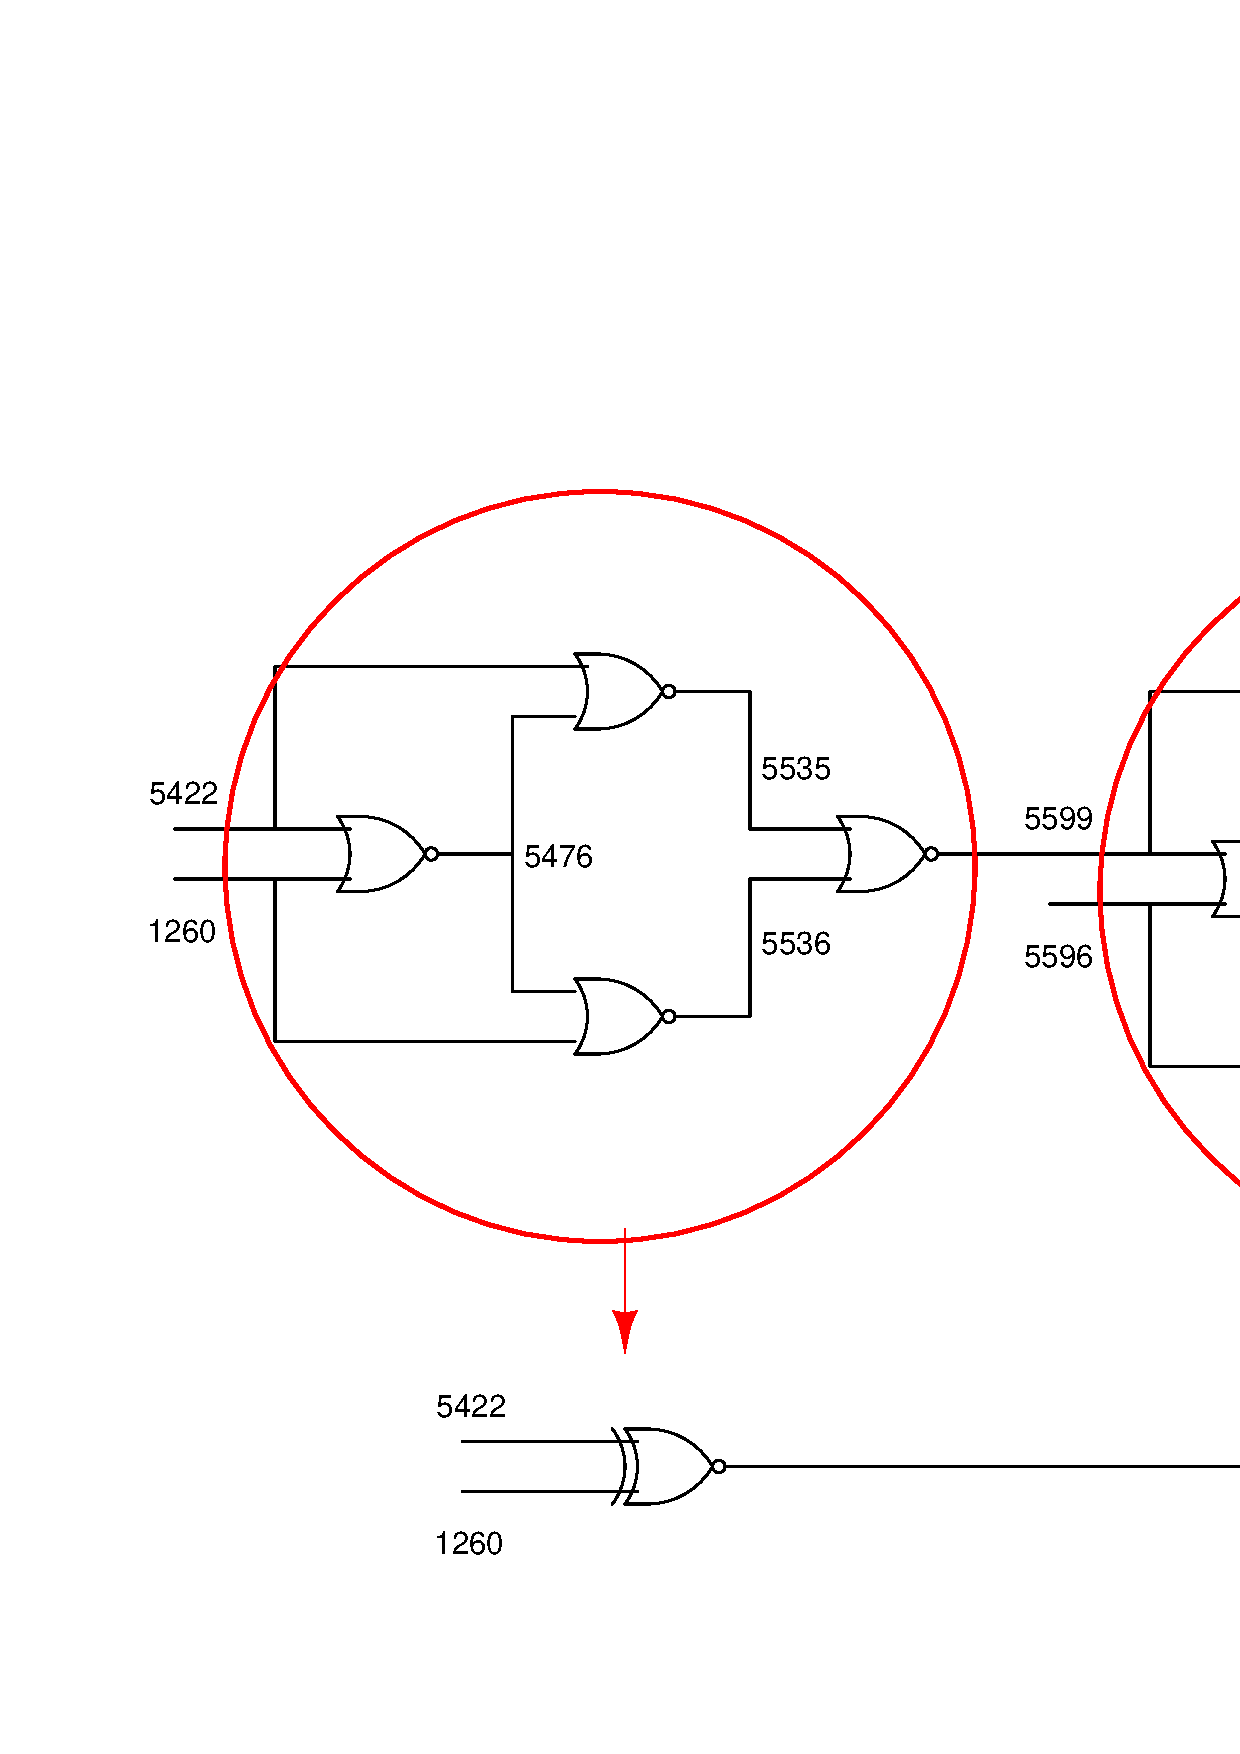
\includegraphics[scale=0.2]{fig/c6288-xor-chains-2.pdf}
                \end{center}
        \end{figure}

\end{frame}

\begin{frame}{\texttt{c499} XOR chains}
       \begin{figure}
                \begin{center}
                \label{fig:c499-c-l}
                \caption{\texttt{c499} XOR chains at primary outputs}
                        \includegraphics[scale=0.2]{fig/c499-xor-chains.pdf}
                \end{center}
        \end{figure}

\end{frame}



\begin{frame}{\texttt{c499} XOR chains}
       \begin{figure}
                \begin{center}
                \label{fig:c499-c-l}
                \caption{\texttt{c499} XOR chains at primary outputs}
                        \includegraphics[scale=0.2]{fig/c499-xor-chains.pdf}
                \end{center}
        \end{figure}

\end{frame}

\begin{frame}{\texttt{c1355} XOR chains}
       \begin{figure}
                \begin{center}
                \label{fig:c1355-c-l}
                \caption{\texttt{c1355} XOR chains at primary outputs}
                        \includegraphics[scale=0.2]{fig/c1355-xor-chains.pdf}
                \end{center}
        \end{figure}

\end{frame}

\begin{frame}{\texttt{c7552} XOR chains}
       \begin{figure}
                \begin{center}
                \label{fig:c7552-c-l}
                \caption{\texttt{c7552} XOR chains at primary outputs}
                        \includegraphics[scale=0.2]{fig/c7552-xor-chains.pdf}
                \end{center}
        \end{figure}

\end{frame}

\begin{frame}{\texttt{c1908} XOR chains}
       \begin{figure}
                \begin{center}
                \label{fig:c1908-c-l}
                \caption{\texttt{c1908} XOR chains at primary outputs}
                        \includegraphics[scale=0.2]{fig/c1908-xor-chains.pdf}
                \end{center}
        \end{figure}

\end{frame}

\begin{frame}{\texttt{c5315} XOR chains}
       \begin{figure}
                \begin{center}
                \label{fig:c5315-c-l}
                \caption{\texttt{c5315} XOR chains at primary outputs}
                        \includegraphics[scale=0.2]{fig/c5315-xor-chains.pdf}
                \end{center}
        \end{figure}

\end{frame}

\begin{frame}{Akash feedback on 20.09.2018}
\begin{itemize}
\item Algorithm to automatically identifying combinational XOR-chains at primary outputs, and encrypting them
\item Algorithm to encrypt the scan-chain
\item Quantify runtime and functional output corruption
\item Implementation on ISCAS'85 and OpenSPARC circuits
\item \alert{Idea}: Since there are primary output XOR-chains for ALUs (used for PC, Branch target calculator, Execution units etc.), this idea will lock the processor successfully
\item Algorithm for selective flip-flop locking, to minimize area overhead due to sequential locking
%\item Target DAC (if more algorithmic work involved) or HOST
\end{itemize}
\end{frame}

\begin{frame}{Next steps}
\begin{itemize}
%\item For selectively locking flip-flops, are some flip-flops more special than others to lock (in terms of shooting-up SAT-running-time and thus making decryption harder) ?
\item Algorithm to decode correct combinational key, given sequential key
\end{itemize}
\end{frame}

\begin{frame}{Algorithm to decrypt correct combinational key}
\begin{itemize}
\item Step 1: Run SAT solver on scan-unrolled combinational circuit, to find sequential key
\item Step 2: Isolate combinational circuit, apply combinational portion of key, and add virtual key gates at POs, and run SAT solver
\item Step 3: Apply virtual key values, and make combinbational key unknown again, and run SAT-solver
\end{itemize}
\end{frame}

\begin{frame}{\texttt{c17} circuit}
       \begin{figure}
                \begin{center}
                \label{fig:c17-c}
                \caption{\texttt{c17} combinational circuit}
                        \includegraphics[scale=0.3]{fig/c17_original.pdf}
                \end{center}
        \end{figure}
\end{frame}

\begin{frame}{\texttt{c17} circuit with sequential locking}
       \begin{figure}
                \begin{center}
                \label{fig:c17-s-l}
                \caption{\texttt{c17} circuit with sequential locking}
                        \includegraphics[scale=0.3]{fig/c17_sequentially_locked.pdf}
                \end{center}
        \end{figure}
\end{frame}


\begin{frame}{\texttt{c17} circuit with scan unroll and Step 1}
       \begin{figure}
                \begin{center}
                \label{fig:c17-s-l-Algo-Step1}
                \caption{\texttt{c17} circuit with scan unroll and Step 1}
                        \includegraphics[scale=0.3]{fig/c17_sequentially_locked_scan_unrolled_Algo_Step1.pdf}
                \end{center}
        \end{figure}
\end{frame}

\begin{frame}{\texttt{c17} circuit with scan unroll and Step 2}
       \begin{figure}
                \begin{center}
                \label{fig:c17-s-l-Algo-Step2}
                \caption{\texttt{c17} circuit with scan unroll and Step 2}
                        \includegraphics[scale=0.3]{fig/c17_sequentially_locked_scan_unrolled_Algo_Step2.pdf}
                \end{center}
        \end{figure}
\end{frame}

\begin{frame}{\texttt{c17} circuit with scan unroll and Step 3}
       \begin{figure}
                \begin{center}
                \label{fig:c17-s-l-Algo-Step2}
                \caption{\texttt{c17} circuit with scan unroll and Step 3}
                        \includegraphics[scale=0.3]{fig/c17_sequentially_locked_scan_unrolled_Algo_Step3.pdf}
                \end{center}
        \end{figure}
\end{frame}

\begin{frame}{Observation}
\begin{itemize}
\item In principle, the Algorithm can solve for the correct combinational key
\item However, we do not have the reference correct combinational circuit for Step 2, since we only have access to scan data on the activated IC
\item Hence Algorithm is not feasible
\item Thus, we need to make $2^M$ (for circuit with M flip-Flops) observations. 
\item For \texttt{c880} circuit, $M=26$, thus running time = $2^{26}*0.04s = 3, 355, 433 s  \approx 1 month $
\item \texttt{c880} has 105 primary inputs (PIs); if we add flip-flops at PIs as well, running time increases $2^{105}\times$ further. 
\end{itemize}
\end{frame}


\begin{frame}{Experimental evaluation}
\begin{itemize}
\item Formulate the sequential locking problem, as an instance of the logic locking problem, and solve for the sequential key
\item Extract the combinational portion of the key, and apply to the combinational portion of the circuit, and check if it is formally equivalent to original circuit
\item If \alert{YES}, it means decrypted decrypted key produces \alert{correct} functional outputs when applied to the encrypted circuit
\item If \alert{NO}, it means decrypted decrypted key produces \alert{corrupt} functional outputs when applied to the encrypted circuit
\end{itemize}
\end{frame}

\begin{frame}{Results for $5\%$ combinational (random) encryption and encrypting all output flip-flops}
\begin{itemize}
\item Decrypted key produces correct functional outputs : \texttt{apex2}, \texttt{apex4}, \texttt{c432}, \texttt{c499} 
\item Decrypted key produces corrupt functional outputs : \texttt{c880}, \texttt{c7552}, \texttt{c1908}, \texttt{c1355}, \texttt{c5315}, \texttt{c2670}, \texttt{c3540}, \texttt{dalu}, \texttt{des}, \texttt{ex1010}, \texttt{ex5}, \texttt{i4}, \texttt{i7}, \texttt{i8}, \texttt{i9}, \texttt{k2}, \texttt{seq}
\item Success rate : $\frac{17}{21}$ cases \alert{$\approx 81\%$}
%\item \alert{ 100\%} correlation between presence of XOR-type encryption at POs and success in functional output corruption
\end{itemize}

\end{frame}

\begin{frame}{Results for $5\%$ target combinational (random and PO) encryption and encrypting all output flip-flops}
\begin{itemize}
\item Decrypted key produces correct functional outputs : \alert{Nil}
\item Decrypted key produces corrupt functional outputs : \texttt{c880}, \texttt{c7552}, \texttt{c1908}, \texttt{c1355}, \texttt{c5315}, \texttt{c2670}, \texttt{c3540}, \texttt{dalu}, \texttt{des}, \texttt{ex1010}, \texttt{ex5}, \texttt{i4}, \texttt{i7}, \texttt{i8}, \texttt{i9}, \texttt{k2}, \texttt{seq}, \texttt{c432}, \texttt{c499}, \texttt{apex2}, \texttt{apex4}
\item Success rate : $\frac{21}{21}$ cases \alert{$= 100 \%$}
\end{itemize}

\end{frame}

\begin{frame}{Results for $5\%$ combinational (DAC'12 fault analysis based) encryption and encrypting all output flip-flops}
\begin{itemize}
\item Decrypted key produces correct functional outputs : \texttt{i4}, \texttt{i7}, \texttt{i8}, \texttt{i9}, \texttt{apex2}, \texttt{apex4}, \texttt{seq}, \texttt{k2}, \texttt{dalu}, \texttt{ex1010}, \texttt{ex5}, \texttt{des}, \texttt{c432}, \texttt{c499}, \texttt{c7552}, \texttt{c1908}, \texttt{c1355}, \texttt{c3540}
\item Decrypted key produces corrupt functional outputs : \texttt{c880}, \texttt{c5315}
\item \texttt{c2670} run in progress ($> 48$ hours). The SAT-attack paper mentions they could not decrypt this benchmark. 
\item Success rate : $\frac{2}{20}$ cases \alert{$= 10\%$}
%\item \alert{ 100\%} correlation between presence of XOR-type encryption at POs and success in functional output corruption
\end{itemize}
\end{frame}

\begin{frame}{Results for $5\%$ combinational (DAC'12 Fault analysis + PO) encryption and encrypting all output flip-flops}
\begin{itemize}
\item Decrypted key produces correct functional outputs :    \texttt{apex2} (only 3 POs),   
\item Decrypted key produces corrupt functional outputs : \texttt{i4}, \texttt{i7}, \texttt{i8}, \texttt{i9}, \texttt{apex4}, \texttt{k2},  \texttt{seq}, \texttt{dalu}, \texttt{des},  \texttt{ex1010}, \texttt{ex5}, \texttt{c432}, \texttt{c499}, \texttt{c880}, \texttt{c1355}, \texttt{c3540}, \texttt{c5315}, \texttt{c1908},  \texttt{c7552} 
\item Success rate : $\frac{19}{20}$ cases \alert{$= 95\%$}
%\item \alert{ 100\%} correlation between presence of XOR-type encryption at POs and success in functional output corruption
%\item \textttt{c7552} took 1 hr runtime
\end{itemize}
\end{frame}

\begin{frame}{Results for $5\%$ combinational (IOLTS'14) encryption and encrypting all output flip-flops}
\begin{itemize}
\item Decrypted key produces correct functional outputs : \texttt{apex2}, \texttt{apex4}, \texttt{i4}, \texttt{i7}, \texttt{i8}, \texttt{i9}, \texttt{ex1010}, \texttt{ex5}, \texttt{k2}, \texttt{seq}, \texttt{dalu}, \texttt{des}, \texttt{c432}, \texttt{c499}, \texttt{c1908}, \texttt{c1355}, \texttt{c5315}, \texttt{c7552}, \texttt{c3540}, \texttt{c880}, \texttt{c2670}
\item Decrypted key produces corrupt functional outputs : \alert{Nil}
\item Success rate = $\frac{0}{21}$ cases = \alert{0\%}
%\item In other words 100\% success in decrypting the correct combinational key
%\item Exact (bit-by-bit) combinational key is getting recovered: looks like equivalence classes don't exist in AND-type or OR-type encryption (IOLTS'14)
\end{itemize}
\end{frame}

\begin{frame}{Results for $5\%$ combinational (IOLTS'14 and PO) encryption and encrypting all output flip-flops}
\begin{itemize}
\item Decrypted key produces correct functional outputs :  \alert{Nil}  
\item Decrypted key produces corrupt functional outputs :  \texttt{c2670}, \texttt{c3540}, \texttt{c5315}, \texttt{c7552}, \texttt{k2}, \texttt{seq}, \texttt{ex5}, \texttt{ex1010},  \texttt{apex2}, \texttt{apex4}, \texttt{c432}, \texttt{c499}, \texttt{c880}, \texttt{i4},  \texttt{i7}, \texttt{i8},  \texttt{i9},  \texttt{c1908}, \texttt{c1355}, \texttt{dalu}, \texttt{des}
\item Success rate = $\frac{21}{21}$ cases = \alert{100\%}
%\item In other words 100\% success in decrypting the correct combinational key
%\item Exact (bit-by-bit) combinational key is getting recovered: looks like equivalence classes don't exist in AND-type or OR-type encryption (IOLTS'14)
\end{itemize}
\end{frame}

\begin{frame}{Results for $5\%$ combinational (TOC13'XOR) encryption and encrypting all output flip-flops}
\begin{itemize}
\item Decrypted key produces correct functional outputs :  \texttt{i9}, \texttt{des}, \texttt{c432}, \texttt{c499}, \texttt{c3540}, \texttt{c880}, \texttt{c1908}
\item Decrypted key produces corrupt functional outputs : \texttt{apex2}, \texttt{apex4}, \texttt{i4}, \texttt{i7}, \texttt{i8}, \texttt{ex1010}, \texttt{ex5}, \texttt{k2}, \texttt{seq}, \texttt{dalu}, \texttt{c1355}, \texttt{c5315}, \texttt{c2670}, \texttt{c7552} 
\item Success rate = $\frac{14}{21}$ cases \alert{$\approx 67\%$}
%\item \alert{ 100\%} correlation between presence of XOR-type encryption at POs and success in functional output corruption
%\item For \texttt{c1355}, no XOR-type key-gate right at PO. 
%\item For \texttt{c7552}, 11 hrs runtime
\end{itemize}
\end{frame}


\begin{frame}{Results for $5\%$ combinational (TOC13'XOR and PO) encryption and encrypting all output flip-flops}
\begin{itemize}
\item Decrypted key produces correct functional outputs :  \alert{Nil}  
\item Decrypted key produces corrupt functional outputs : \texttt{apex2}, \texttt{apex4}, \texttt{i4}, \texttt{i7}, \texttt{i8}, \texttt{ex1010}, \texttt{ex5}, \texttt{k2}, \texttt{seq}, \texttt{dalu}, \texttt{c1355}, \texttt{c5315}, \texttt{c2670}, \texttt{c7552}, \texttt{i9}, \texttt{c432}, \texttt{c499}, \texttt{c1908}, \texttt{c880}, \texttt{c3540}, \texttt{des},
\item Success rate = $\frac{21}{21}$ cases \alert{$= 100\%$}
\end{itemize}
\end{frame}


\begin{frame}{Results for $5\%$ combinational (TOC13'MUX) encryption and encrypting all output flip-flops}
\begin{itemize}
\item Decrypted key produces correct functional outputs : \texttt{apex2}, \texttt{i4}, \texttt{i7}, \texttt{i8}, \texttt{i9}, \texttt{ex1010}, \texttt{ex5}, \texttt{k2}, \texttt{seq}, \texttt{dalu}, \texttt{des}, \texttt{c432}, \texttt{c499}, \texttt{c1355}, \texttt{c5315}, \texttt{c7552}, \texttt{c3540}, \texttt{c2670}, \texttt{c880}, \texttt{c1908}
\item Decrypted key produces corrupt functional outputs : \texttt{apex4}
\item Success rate = $\frac{1}{21}$ cases \alert{$\approx 5\%$}
\end{itemize}
\end{frame}

\begin{frame}{Results for $5\%$ combinational (TOC13'MUX and PO) encryption and encrypting all output flip-flops}
\begin{itemize}
\item Decrypted key produces correct functional outputs : \alert{Nil}
\item Decrypted key produces corrupt functional outputs : \texttt{apex4}, \texttt{apex2}, \texttt{i4}, \texttt{i7}, \texttt{i8}, \texttt{i9}, \texttt{ex1010}, \texttt{ex5},  \texttt{k2}, \texttt{seq},  \texttt{dalu},  \texttt{des} ($\approx$ 2 hours), \texttt{c432}, \texttt{c499}, \texttt{c1355}, \texttt{c5315}, \texttt{c880}, \texttt{c1908}, \texttt{c3540}, \texttt{c7552}, \texttt{c2670}, 
\item Success rate = $\frac{21}{21}$ cases \alert{$\approx 100 \%$}
\end{itemize}
\end{frame}

%\begin{frame}{Complexity to decrypt correct combinational key}
%\begin{itemize}
%\item If circuit $C$ has $M$ POs, search-space to explore which outputs undergo inversions along scan-chain and which not, is \alert{$2^M$}.
%\item Because of this exponential search-space and typical circuits can have hundreds of POs, it is not possible for SAT-attacker to decrypt correct combinational key, given the decrypted sequential key.
%\end{itemize}
%\end{frame}

\begin{frame}{Theorem}
Using virtual gates (shown in slide 62), it is possible to find portion of correct combinational key (except the encryption bits at POs)
\end{frame}

\begin{frame}{Theorem}
It is not possible to find the encryption bits at POs
\end{frame}

\begin{frame}{Conclusion}
Hence, our methodology in adding XOR-based encryption gates at POs, is ROBUST (in the sense that it is not possible to reformulate and solve for the PO encryption key bits, hence not possible to decrypt the complete combinational key). 
\end{frame}

\begin{frame}{Boundary Encryption- Experiment 1}
\begin{itemize}
\item I have added XOR-type encryption key gates to all 7 outputs of \texttt{c432} circuit and encrypted all output flip-flops
\item The {\em functionally correct key} is \alert{0000000} (singleton equivalence class)
\item However, running ScanSAT on scan unrolled version of above boundary encrypted \texttt{c432} circuit, gave \alert{0010000}, hence corrupting functional output
\item Thus, boundary encryption produces SAT-attack Resilient Circuits. 
\item No need to add key gates deep inside combinational logic. 
\end{itemize}
\end{frame}


\begin{frame}{Boundary Encryption- Experiment 2}
\begin{itemize}
\item Everything same as experiment 1, however number of encrypted POs is variable
\item {7, 6, 5, 4, 3, 2}: decrypted \alert{functionally incorrect key}
\item {1} : decrypted {functionally correct key}
\item So, minimum 2 POs need to be encrypted. This is what I have manually done in all the experiments, across the 21 benchmarks, spanning the 5-encryption-schemes. Hence, the success rate reached \alert{100 \%} by just encrypting just 2-3 POs. 
\end{itemize}
\end{frame}

\begin{frame}{Advantages of Boundary Encryption}
\begin{itemize}
\item We need to add few XOR/XNOR-type encryption key gates, just at POs, and no need to add them deep inside combinational logic. 
\item This makes the encryption scheme very area-efficient. The key gates can be added to timing-uncritical POs. 
\item Area, Timing and Power friendly. 
\item This makes this method seamless integrable to industry practice
\item The method scales easily from IP-level to SoC-level. 
\end{itemize}
\end{frame}

\begin{frame}{Advantages of Boundary Encryption/Locking}
\begin{itemize}
\item Logic Locking techniques lock only the combinational logic, hence vulnerable to scan-based SAT-attack, EDT-Bypass mode; 
\item Scan Locking locks only the scan chains, using Encrypt-Flip-Flop. However, ScanSAT models this as an instance of logic locking problem, hence also vulnerable to SAT-attack; 
\item \alert{Boundary Locking} combines both intelligently, to thwart SAT-attack. 
\item Compare area overhead for all circuits reported in Table II of Encrypt Flip-Flop paper. 
\item Report running times
\end{itemize}
\end{frame}

%\begin{frame}[allowframebreaks]
\frametitle<presentation>{References}

\begin{thebibliography}{1}

\bibitem{halter:97}
J.P. Halter, F.N. Najm, ``A gate-level leakage power reduction method for ultra-low-power CMOS circuits'',  Custom Integrated Circuits Conference, IEEE, 1997, pp.475-478.

\bibitem{yibin:98}
Y. Ye, S. Borkar, and V. De, ``A new technique for standby leakage reduction in high-performance circuits,'' Symposium on VLSI Circuits, IEEE, 1998, pp. 40-41.

\bibitem{tschanz:03}
J.W. Tschanz, S.G. Narendra, Y. Ye, B.A. Bloechel, S. Borkar, and V. De, ``Dynamic sleep transistor and body bias for active leakage power control of microprocessors,'' IEEE Journal of Solid-State Circuits, vol. 38, Nov. 2003, pp. 1838-1845.

\bibitem{usami:06}
K. Usami and N. Ohkubo, ``A Design Approach for Fine-grained Run-Time Power Gating using Locally Extracted Sleep Signals,'' International Conference on Computer Design, IEEE, 2006, pp. 155-161.

\bibitem{bhunia:05}
S. Bhunia, N. Banerjee, Q. Chen, H. Mahmoodi, and K. Roy, ``A novel synthesis approach for active leakage power reduction using dynamic supply gating,'' Design Automation Conference, IEEE, 2005, pp. 479-484.

\bibitem{leinweber:08}
L. Leinweber and S. Bhunia, ``Fine-Grained Supply Gating Through Hypergraph Partitioning and Shannon Decomposition for Active Power Reduction,'' Design, Automation and Test in Europe, IEEE, 2008, pp. 373-378.

\bibitem{borkar:06}
S. Borkar, ``Tackling variability and reliability challenges'', IEEE Design and Test of Computers, vol.23, no.6, 2006, pp.520

\bibitem{rohfleisch:96}
B. Rohfleisch, A. Kolbl, B. Wurth, ``Reducing power dissipation after technology mapping by structural transformations'', Design Automation Conference Proceedings , IEEE, 1996, pp.789-794.

\end{thebibliography}
\end{frame}



\section{}
\begin{frame}
\begin{center}
Thank you! 
\end{center}
\end{frame}

\end{document}
